%!TEX program = <xelatex>
\documentclass{book}
\usepackage{mystyle}
\begin{document}

In this Chapter we motivate the use of the \PT\, making use of an example widely-cited in the literature,see \cite{BaragattiParallelTemperingWithEquiEnergyMoves} and \citet*{FamingLiang}. 

As pointed out in the Introduction, the reason for using the \PT\, is the multimodiality of the distribution of interest, $\pi$. In our simulations we assume to know the density function of $\pi$ to be the following mixture of normal densities:

\begin{equation}\label{experimental pi}
f(x) = 
\sum_{i=1}^{20} \frac{\omega_i}{ \sigma_i \sqrt{2 \pi} } \exp \Big( -\frac{(x - \mu_i)^\tran (x - \mu_i)}{2 \sigma_i^2} \Big),	
\end{equation}
where $\sigma_1 = \dots = \sigma_{20} = 0.1$, $\omega_1 = \dots = \omega_{20} = 0.05 $, and where  the means $\mu_i$ are given by

\begin{table}[ht]
	\centering
\begin{tabular}{rrrrrrrrrr}
  \hline
$\mu_1$ & $\mu_2$ & $\mu_3$ & $\mu_4$ & $\mu_5$ & $\mu_6$ & $\mu_7$ & $\mu_8$ & $\mu_9$ & $\mu_{10}$ \\ 
  \hline
2.18 & 8.67 & 4.24 & 8.41 & 3.93 & 3.25 & 1.70 & 4.59 & 6.91 & 6.87 \\ 
  5.76 & 9.59 & 8.48 & 1.68 & 8.82 & 3.47 & 0.50 & 5.60 & 5.81 & 5.40 \\ 
   \hline
\end{tabular}
\end{table}
and 

\begin{table}[ht]
	\centering
\begin{tabular}{rrrrrrrrrr}
  \hline
$\mu_{11}$ & $\mu_{12}$ & $\mu_{13}$ & $\mu_{14}$ & $\mu_{15}$ & $\mu_{16}$ & $\mu_{17}$ & $\mu_{18}$ & $\mu_{19}$ & $\mu_{20}$ \\ 
  \hline
5.41 & 2.70 & 4.98 & 1.14 & 8.33 & 4.93 & 1.83 & 2.26 & 5.54 & 1.69 \\ 
  2.65 & 7.88 & 3.70 & 2.39 & 9.50 & 1.50 & 0.09 & 0.31 & 6.86 & 8.11 \\ 
   \hline
\end{tabular}
\end{table}
 
Figure \ref{ToyExample} inspects visually the density. One notices easily that different peaks get intermingled, as only $15$ peaks are visibleout of $20$ peaks are clearly visible. The peaks are usually seperated by at least an area of unit diameter of lowered probability mass.   

\begin{figure}
	\begin{minipage}[b]{.5\linewidth}
		\centering 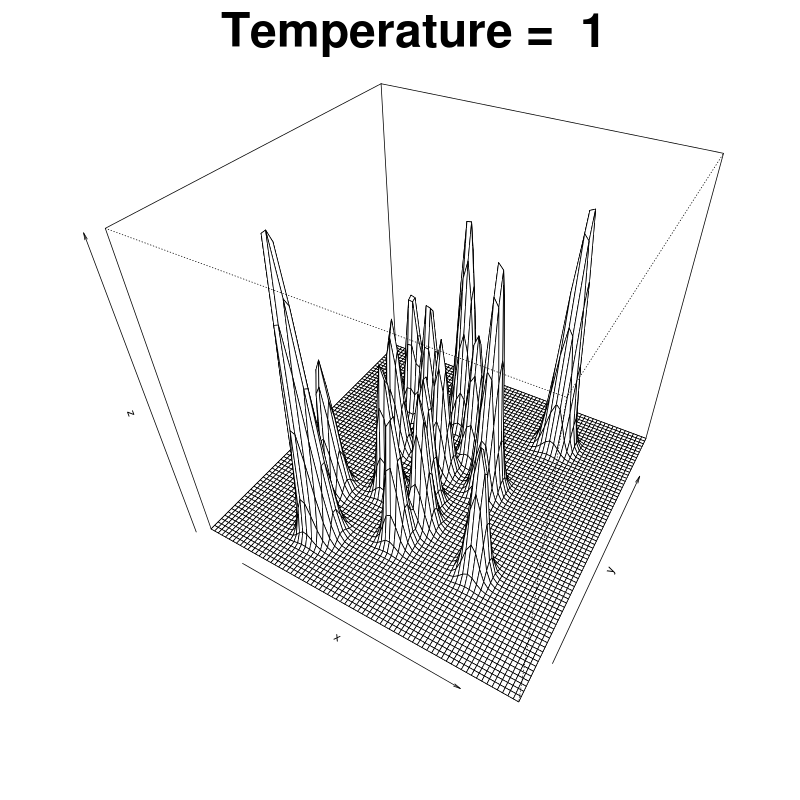
\includegraphics[scale=.25]{./img/Liang_perspective.png}
		\subcaption{Perspective view}\label{LiangContour}
	\end{minipage}%
	\begin{minipage}[b]{.5\linewidth}
		\centering 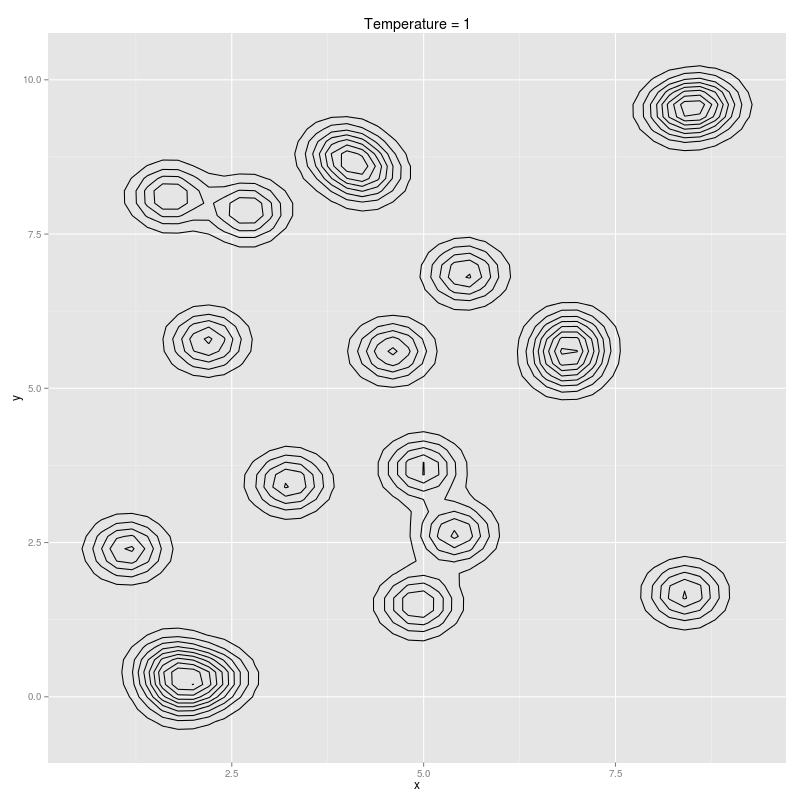
\includegraphics[scale=.25]{./img/Liang_Contour_plot.png}
	\subcaption{Level-set view}\label{LiangPerspective}
	\end{minipage}
	\caption{Toy-example density.}\label{ToyExample}
\end{figure}

The \MH\, is known to be a local algorithm and the reasons for it will be exposed in Chapter \ref{theory}. To motivate the use of the \PT\, it is enough to say for now that sample points generated by the usual \MH\footnote{For introduction to the theory behind the Metropolis-Hastings algorithm consider \cite{CharlesJ.Geyer}.} will be more often drawn from the vicinity of modes. This in turn might give the impression that most of the probability is concentrated somewhere next to the starting points\footnote{We choose the starting points at random}. We shall refer to the percentages of iterations in the vicinity of a particular mode its sojourn time, postponing a more thorough definition till Chapter \ref{simulationsAndResults}. 

By the results that stem from the Ergodic Theory, the sojourn times for each component of the mixture given by Eq. \ref{experimental pi} should converge to the probabilities of the modes' vicinity areas, $\omega_i$, and so be roughly equal in the above-mentioned example. However, in practical terms, this convergence might be prohibitively long, way longer than what a typical user would consider fortunate to wait for. This is clearly a big problem, since in practical applications, as mentioned in the \ref{Introduction}, one considers the approximation of the needed integral to be simply the mean evaluation of a function on the generated sample point and these approximations cannot possibly be good if we cut the procedures too quickly. 

To investigate the \MH's localness, we have run the \Metro\, routine. Figures \ref{unexploredShort} and \ref{unexploredLong} show that the localness of the algorithm is persistent even with longer runs of the \MH, the reasons for which will be mentioned in Chapter \ref{theory}. Of course any type of inference based on results based on sample points as in Figure \ref{unexploredLong} would be totally not true.  

\begin{figure}
	\begin{minipage}[b]{.5\linewidth}
		\centering 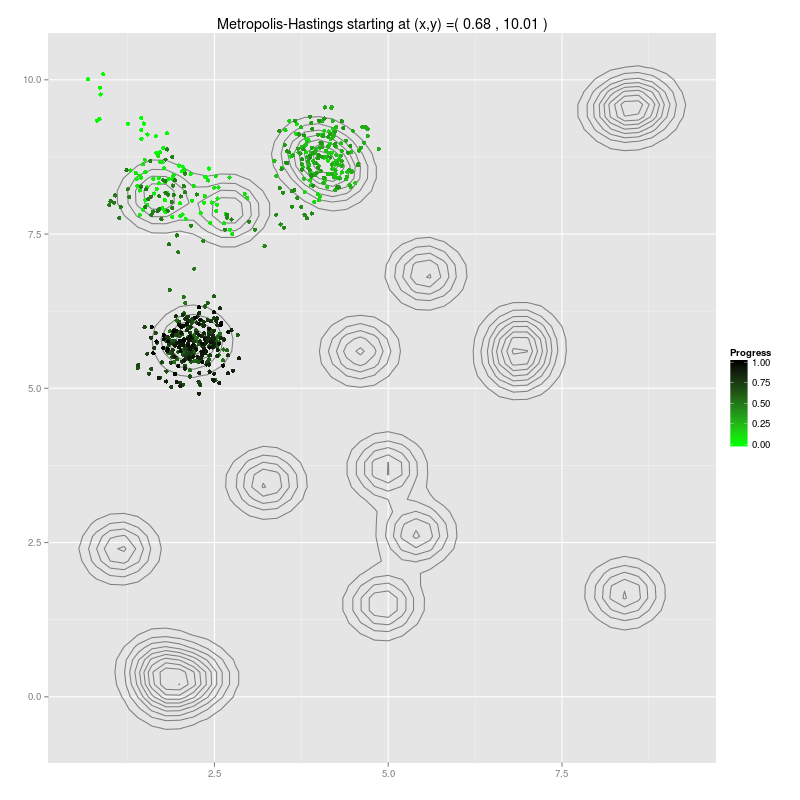
\includegraphics[scale=.25]{./img/MH_simululation_1000_steps_ex1.png}
		\subcaption{Thousand steps\dots}
	\end{minipage}%
	\begin{minipage}[b]{.5\linewidth}
		\centering 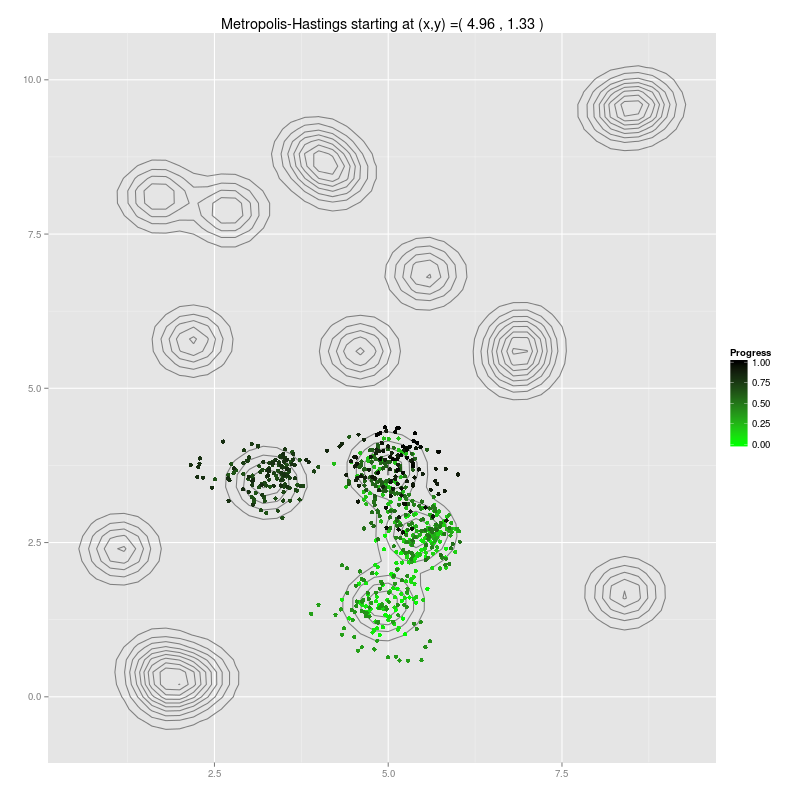
\includegraphics[scale=.25]{./img/MH_simululation_1000_steps_ex2.png}
	\subcaption{\dots that lead nowhere.}
	\end{minipage}
	\caption[Thousand Iterations of \MH]{Thousand Iterations of \MH\,- about $250$ different points generated. Colour intensity increases as points get generated in more advanced stages of the algorithm. One notices easily that short runs of the algorithm do not explore the whole \sspace.}\label{unexploredShort}
\end{figure}


\begin{figure}[ht]
	\centering 
	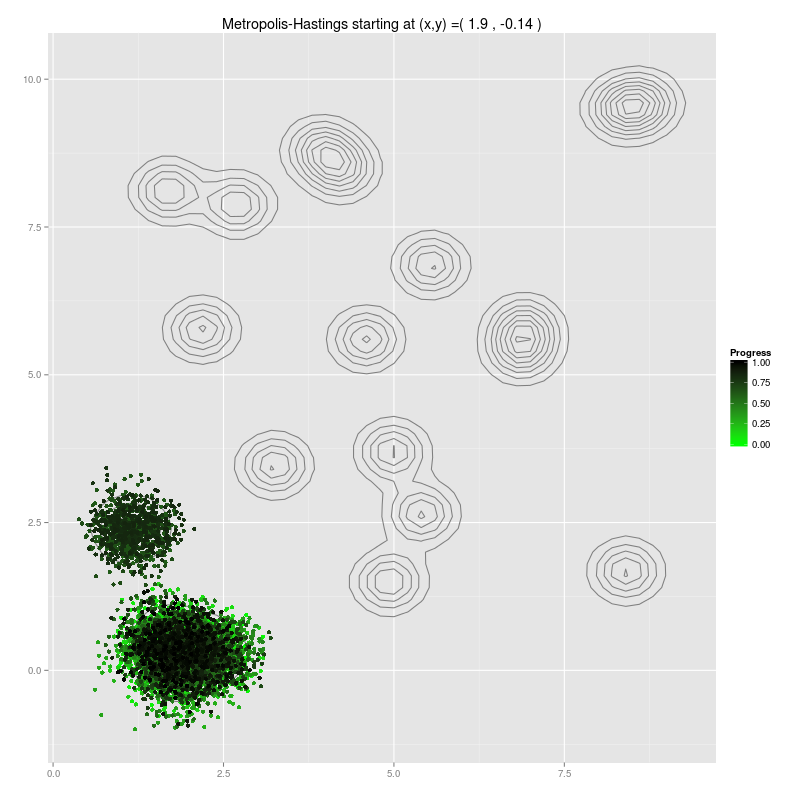
\includegraphics[width=.5\textwidth,keepaspectratio]{./img/MH_simululation_10000_steps.png}
	\caption[]{Ten Thousand Iterations of \MH\,- about a quarter of which resulted in different points. Again the \MH\, failed at exploring the whole \sspace.}\label{unexploredLong}
\end{figure}


Everything changes when one considers the \PT\, instead, as seen in Figures \ref{PTshort} and \ref{PTlong}. In Figure \ref{plotStrategy1} one can visually ascertain himself that most of the \sspace\,got explored. In Figure \ref{plotStrategy2} one notices that only one mode was never explored. The simulation however was not a very long one. If one sets the number of iterations to be higher there are no modes that are unexplored in the studied example, as shown in Figure \ref{PTlong}. In this picture one notices clearly that points accumulate in the regions with higher probability levels.  

\begin{figure}
	\begin{minipage}[b]{.5\linewidth}
		% \centering 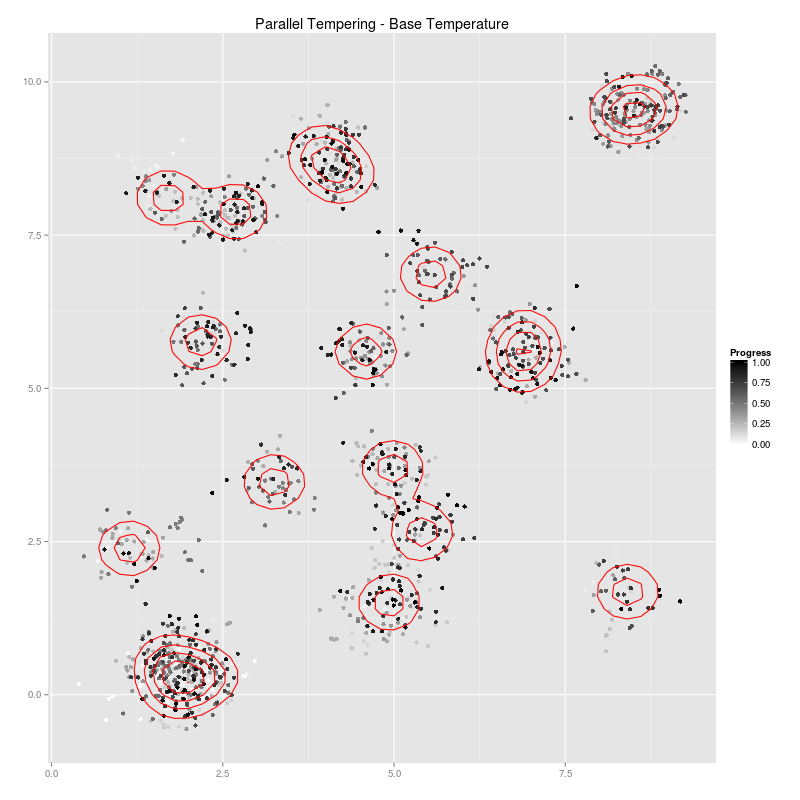
\includegraphics[scale=.25]{./img/PT_simululation_base_temperature_2000_steps_strategy_1_try_1.png}
		\centering 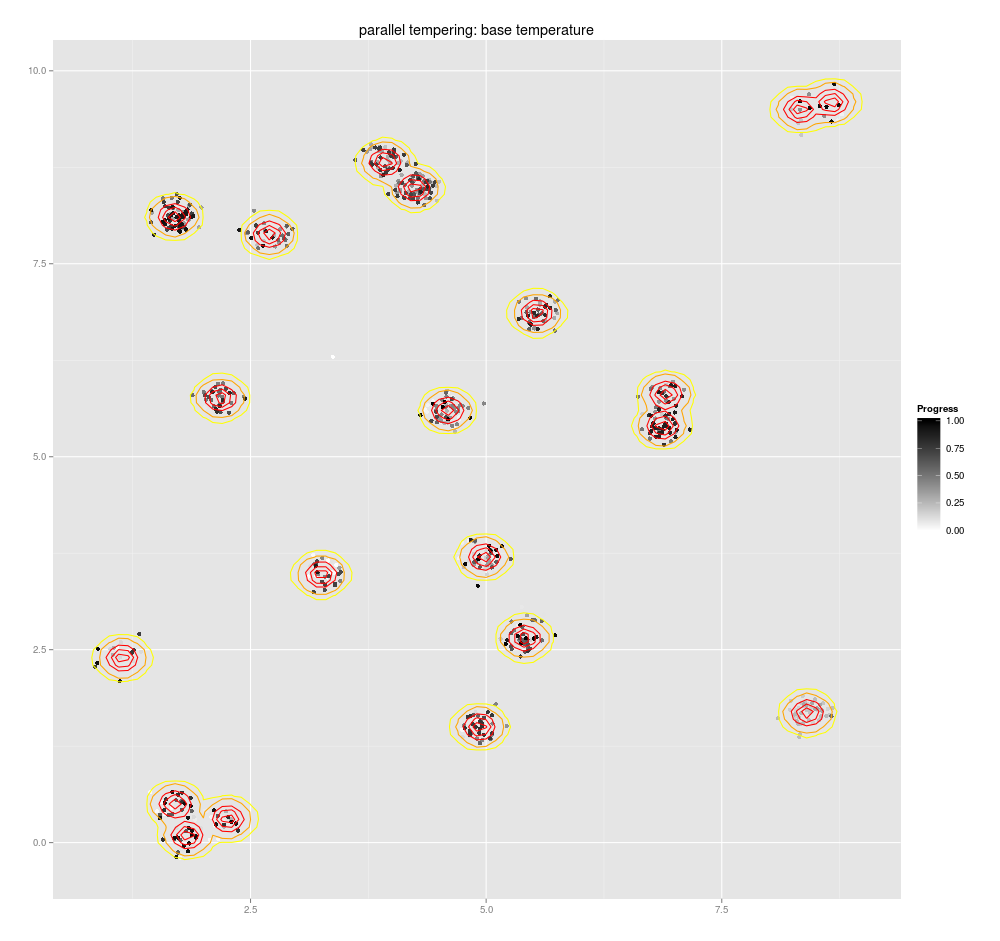
\includegraphics[width=\textwidth, keepaspectratio=true]{./img/strat1with2000it.png}
		\subcaption{Two thousand steps under \strat\,1.\dots}\label{plotStrategy1}
	\end{minipage}%
	\begin{minipage}[b]{.5\linewidth}
		% \centering 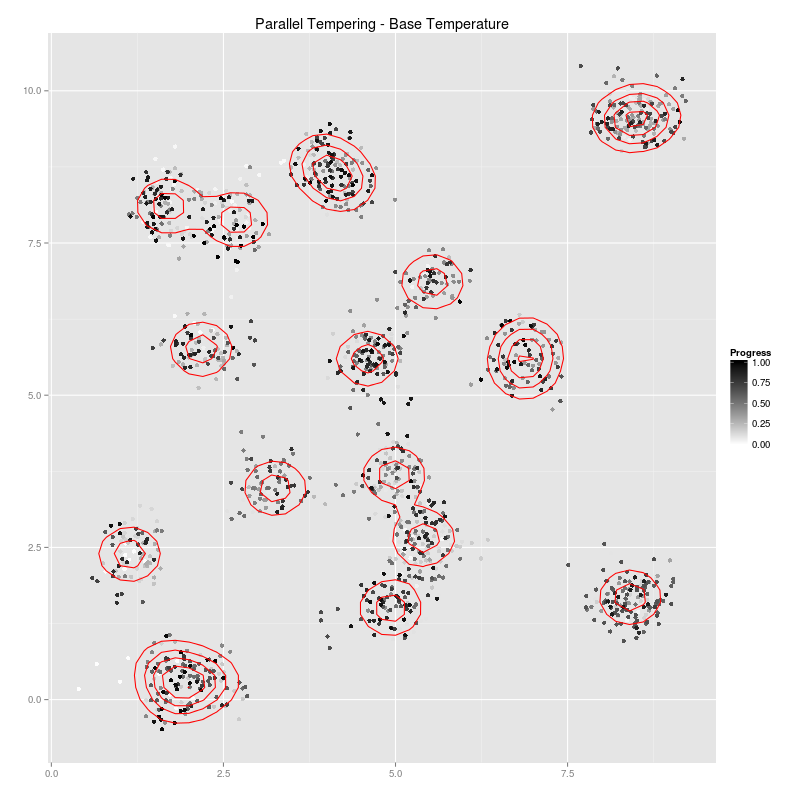
\includegraphics[scale=.25]{./img/PT_simululation_base_temperature_2000_steps_strategy_2_try_1.png}
		\centering 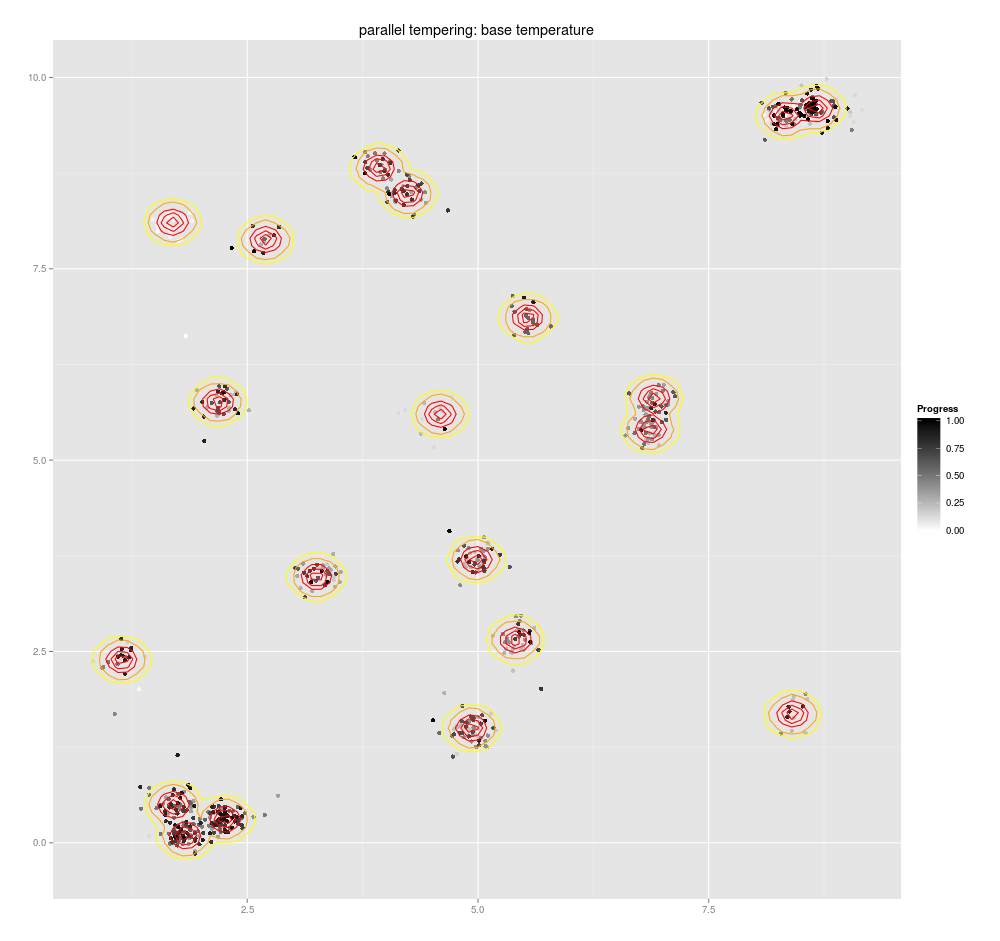
\includegraphics[width=\textwidth, keepaspectratio=true]{./img/strat2it2000.png}		
	\subcaption{Two thousand steps under \strat\,2.}\label{plotStrategy2}
	\end{minipage}
	\caption[\PT\, with \strat\,1 and \strat\,2]{Results of the \PT\,when  and \strat\,2 from Chapter \ref{theory} are applied. One notices immediately the qualitative difference between these examples and the \MH\,results, as the \sspace\, is explored more thouroughly. The results are obtainable under a minute on a modern computer equiped with one core processor unit, 1.5 GHz.}\label{PTshort}
\end{figure}

\begin{figure}[ht]
	\centering 
	% 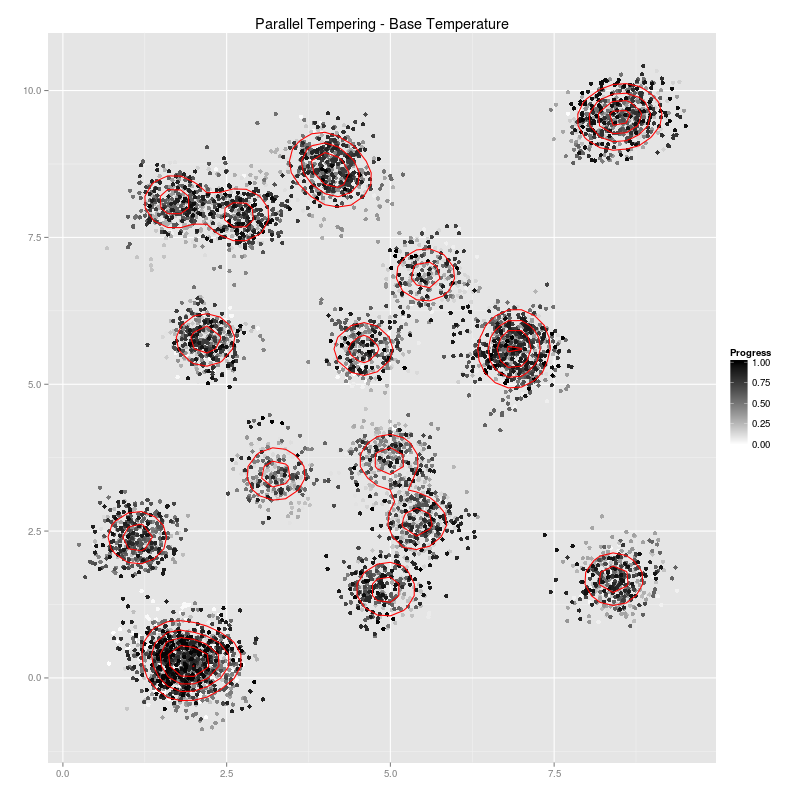
\includegraphics[width=\textwidth,keepaspectratio]{./img/PT_simululation_base_temperature_10000_steps_1.png}
	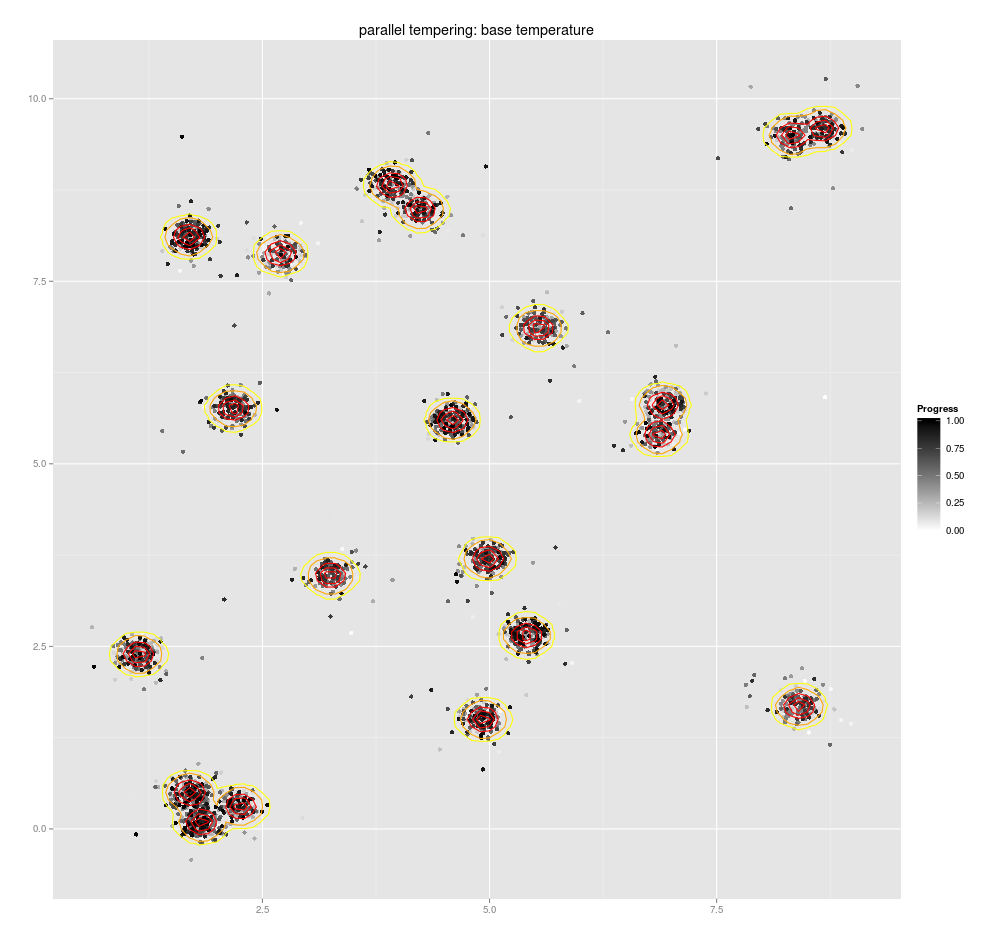
\includegraphics[width=\textwidth,keepaspectratio]{./img/PT10000Motivation.png}
	\caption[Ten Thousand Iterations of \PT]{Ten Thousand Iterations of \PT\, with 2500 iterations of burn-in, under \ref{strat3}. About a quarter of random-walk steps were accepted. The simulation lasted about 140 seconds on a 8 years-old computer equiped with a one core computer. The isoquants encircle regions that contain one percent of overall probability mass (in yellow), five percent (orange), and twenty five, fifty and seventy five (all in red). The shading of sample points varies from white to black, getting darker as the simulation proceeds.}\label{PTlong}
\end{figure}

\end{document}

.01, .05, .25, .5, .75